\chapter{Fifth Species of Counterpoint}\label{ch:5SP}
% Introduction to what is the 5th species of counterpoint
% What is different from other species
% - there is no real constraint (exception: "double croche" cannot deal with that with the actual architecture)
% - each note constraints comes from another species
% - you cannot search for a solution with each species and then merge them somehow because you lose the flexibility of the 5th species
% - constraints cannot be removed after being added so it has to be dynamically linked into the csp
% Species array system
% - constraints (add reify for all constraints, make all constraints act like that and add a TRUE boolean array by default)
% - complex constraints (dissonance when thesis is syncopated)
% - rhythm constraints (0 3 4)
% - dealing with an array with all the notes (same solution avoided)
% - parser
The fifth species of counterpoint, also called \emph{florid counterpoint}, consists of a combination of the four preceding species but mainly of the third and fourth. Indeed, a florid counterpoint in Fux's work looks like an alternation between quarter notes and syncopations, with a few shorter syncopations and eighth notes (binding quarter notes). It is more uncommon to find half notes and it is difficult to determine whether they come from the second or the fourth species.
\begin{figure}[h]
    \centering
    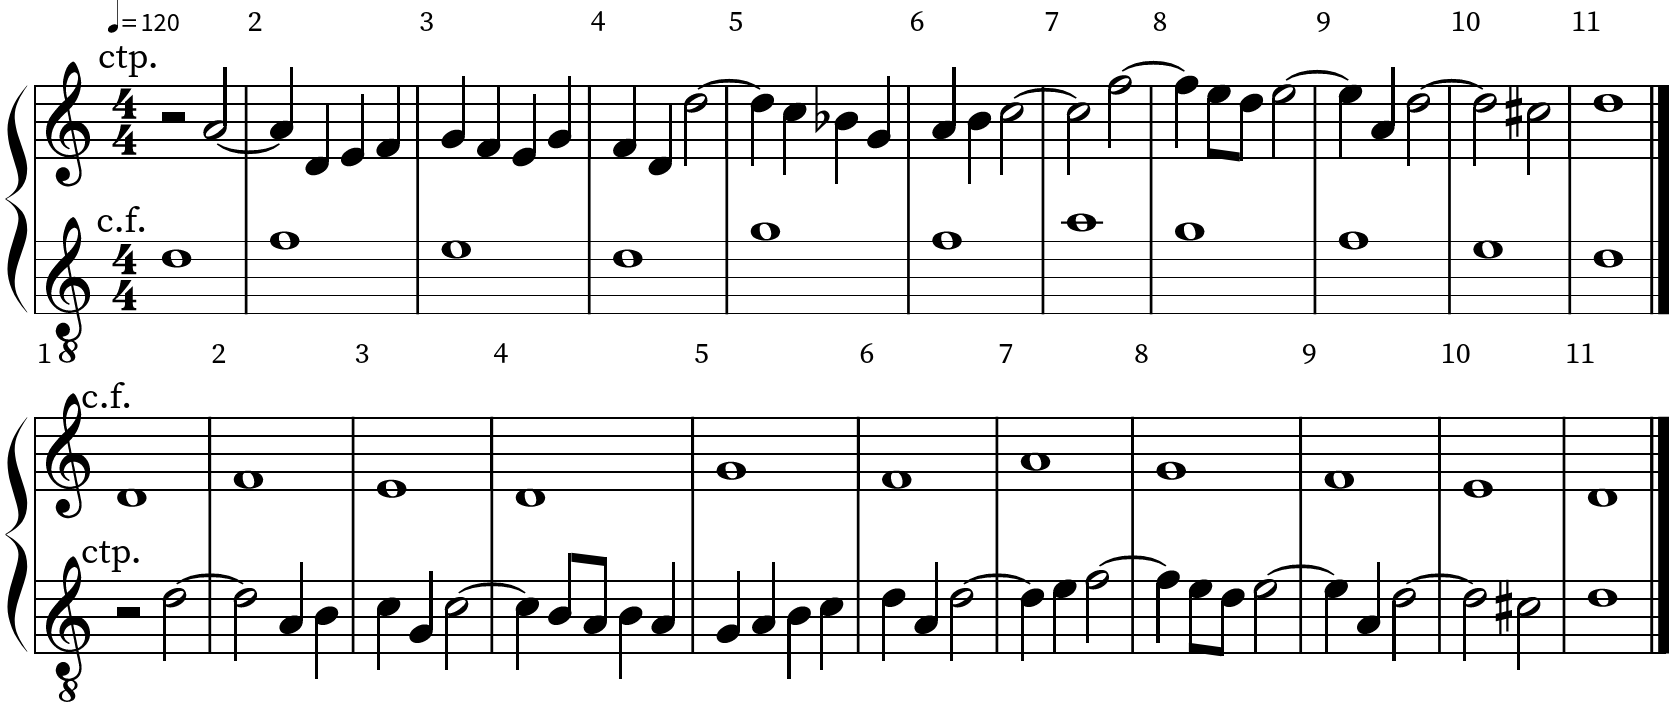
\includegraphics[width=5in]{Images/the_fifth_species.png}
    \caption{Two florid ctp. \listen{Listen5SP} \listenyt{https://youtu.be/9yB4OGr4Cgk?t=231}}
\end{figure}

The florid counterpoint is much free than its predecessors because the number of possibilities increases drastically with the possibility of adapting the species and thus the rhythm and the rules to obtain certain notes more easily than with the previous species. Here, more flexibility means easier to find a solution but more possibilities to explore for the solver. It is partly for these reasons that this chapter will be completely different from the previous ones. Where the others were formalizations of rules, this one is concerned with another problem: the relations between the different constraints of the previous species and the notion of rhythm that comes from them.

This chapter is mainly intended for computer scientists and mathematicians. This implies that the reader is aware of the different notions established in chapter \ref{ch:Formalization} and that he understands the role of the variables previously introduced. Where the previous chapters were divided into two parts (natural language and constraints in the form of mathematics), the present chapter develops logic as a whole.

\section{Problem Differences from Previous Species}
Several points differentiate this species from others and influence the approach to be adopted:
\begin{itemize}[wide]
    \item Fux does not describe new rules specific to this species, there are only new constraints linking the third and fourth species together. This is undoubtedly the lesson with the least information about its functioning.
    \item Fux shows variants at syncopations such that the second half note is replaced by a quarter note; and variations on quarter notes by replacing them with eighth notes to fill in third skips or add mordent\footnote{A mordent is a type of ornament referring to a quick alternation between a note and its upper or lower neighbor.\parencite{Mordent}}.
    \item So far, the solver has no notion of rhythm, its only goal was to find a list of note pitches. Now it must also be able to calculate which species are used where so that a rhythm can be deduced.
    \item Since notes must be constrained differently depending on the species they are part of, all species constraints cannot simply be applied to all notes. Furthermore, it is impossible with Gecode to dynamically remove constraints after they have been applied\footnote{It is possible to \emph{add} constraints dynamically after the CSP has been created, but nothing has been found to perform the operation the other way around, which seems much more complex.}. Therefore, another way must be found to have the constraints applied fully dynamically.
\end{itemize}

\section{Representation of Species as Constraints}
As explained before, the only values that had to be calculated and explicitly provided by the solver were the list of MIDI notes that form the generated counterpoint. Since each species only has notes of equal duration (apart from the last note which is necessarily a whole note), there is no constraint determining whether a note must exist or not at a certain position. Moreover, in the lesson of the fifth species Fux gives only too little information on any rhythm to follow to extract hard constraints.

\subsection{Naive Solution}
A naive solution would be to individually generate solutions from the previous species and somehow merge them. The problem with this approach is that the flexibility offered by the fifth species would be lost. Indeed, certain notes of a certain species may be only accessible from the use of a note of another species. Therefore there would be no interaction between the species and the main asset of the solver would be lost, i.e. being able to find a better solution according to preferences and associated costs.

\subsection{Species Array System}
The only approach that seems correct is to create an array of integer variables the same size as the counterpoint array $Cp$. Each variable would then represent which species the note belongs to at the same location in $Cp$. In this case, all the variables will be used, i.e. as many as the number of notes in a counterpoint of the third species containing only quarter notes. If this array determines to which species the corresponding note belongs, it also determines if a note does \emph{not} belong to any species. That is, whether a note at a certain beat of a certain measure exists or not. This is how the notion of rhythm appears. Caution, declaring that a note does not exist implies that it is not in the final result of the counterpoint that the user sees in the interface. But in reality, the note does indeed exist in the space of constraints for the solver. There is an important distinction between the notes displayed to the user and the notes calculated by the solver. All this will be explained in more detail later.\\

A mathematical formalization is necessary. Let $S$ be an array of same size and structure as $Cp$\footnote{Size of $s_m$, composed of four lists each representing a beat over the entirety of the measures, as always.} representing to which species belongs the note at the same index in the array $Cp$.

\begin{equation}
    \begin{gathered}
        \forp\\
        S[\rho] = \begin{cases}
            0 & \text{if } Cp[\rho] \text{ is not constrained by any species}\\
            1 & \text{if } Cp[\rho] \text{ is constrained by the first species}\\
            2 & \text{if } Cp[\rho] \text{ is constrained by the second species}\\
            3 & \text{if } Cp[\rho] \text{ is constrained by the third species}\\
            4 & \text{if } Cp[\rho] \text{ is constrained by the fourth species}\\
        \end{cases}\\
    \end{gathered}
\end{equation}

Without going into details for the moment, the solver never generates solutions with $S[\rho] \in \{1, 2\}$ which gives in the current state a domain equal to $\{0, 3, 4\}$.

\begin{figure}[h]
    \centering
    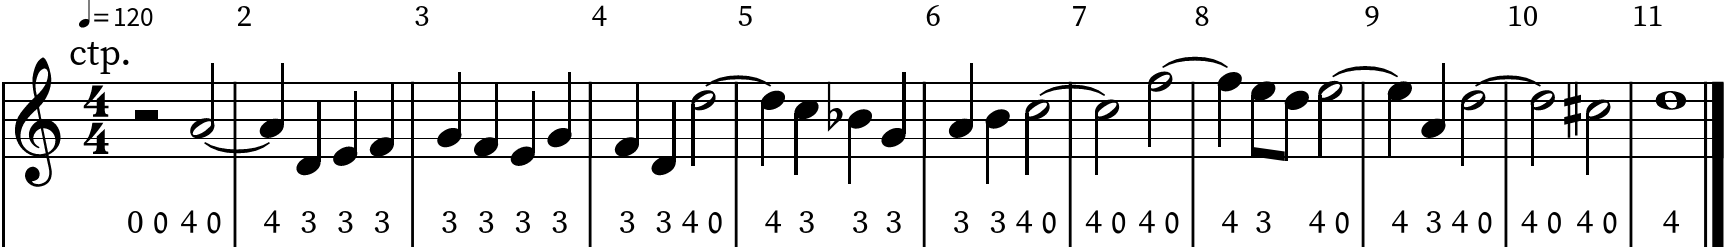
\includegraphics[width=\textwidth]{Images/species_array.png}
    \caption{Representation of the species array $S$ along a ctp., \species{5}.}
    \label{fig:speciesarray}
\end{figure}

By analyzing figure \ref{fig:speciesarray}, one may notice that some patterns are emerging: all syncopations are distinguished by $4-0-4$ while quarter notes are never followed by $0$. These patterns are rhythm constraints imposed in the solver but for now let's leave that and assume that $S$ has coherent values, i.e. syncopations and quarter notes where it is possible to have them.

Now let $IsS_{x}$ be another array of same size and structure as $Cp$ representing whether a note belongs to species $x$ where $x$ is the number assigned to the species in $S$ just above.

\begin{equation}
    \begin{gathered}
        \forall x \in \{0, 1, 2, 3, 4\}, \forp\\
        IsS_{x}[\rho] = \begin{cases}
            \top & \text{if } S[\rho] = x\\
            \bot & \text{otherwise}
        \end{cases}\\
    \end{gathered}
\end{equation}

For example, $IsS_{0}[i, j] = \top$ means that the note at the beat $i$ from the measure $j$ is not contrained by any species. This does not mean that no constraint is placed on this note, only that the constraints of the species placed on this note are in this case necessarily respected. When an $\lor \top$ is added to a constraint, it renders the original constraint useless because the whole thing then becomes a tautology which is equivalent to remove the original constraint.

\section{Formalization of the Species Rhythm into Constraints}
In order for the array $S$ and $IsS$ to have relevant values, i.e. values which respect a format making it possible to produce a coherent rhythm, there must be constraints imposing that certain species may or may not exist at certain positions. These constraints come from common sense and have been created from the examples of the \citetitle{GaPFr}. The context is \emph{no longer} Fux's music theory but computer logic. The first four rules are mandatory for the proper functioning of the system while additional rules have been added to limit the possibilities of rhythm.

\begin{enumerate}[wide, label=\bfseries 5.R\arabic*]
    \item  \label{rhythm:taexist} \textit{There must always be a note in thesis and in arsis, except the very first thesis and the very last arsis.}
    
    No species would allow not to have a note in thesis and only the first species does not have a note in arsis, a species which is not used in florid counterpoint (the last whole note of the counterpoint is the same in all species and is therefore not considered a particularity of any species).
    \begin{equation}
        \begin{gathered}
            \forall j \in [0, m)\\
            \lnot IsS_{0}[0, j]\quad \text{ where } j \neq 0\\
            \lnot IsS_{0}[2, j]\quad \text{ where } j \neq m-1
        \end{gathered}
    \end{equation}

    \item \label{rhythm:no4in2and4} \textit{The \species{4} can only exist in first and third beat.}
    
    Indeed, the notes beginning or ending a syncopation in this species are always located in these beats.
    \begin{equation}
        \begin{gathered}
            \forall i \in \{1, 3\}, \forall j \in [0, m)\quad
            \lnot IsS_{4}[i, j]
        \end{gathered}
    \end{equation}

    \item \label{rhythm:404} \textit{A \species{4} in the third beat necessarily implies a \species{4} in the first beat of the following measure and vice versa. The fourth beat should then have no note.}
    
    This simply describes the usual syncopation which consists of the mandatory $4-0-4$ sequence (see figure \ref{fig:syncimp}).

    \begin{multicols}{2}
        \begin{Figure}
            \centering
            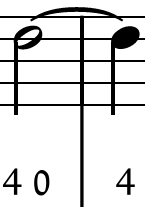
\includegraphics[height=0.8in]{Images/species_404.png}
            \captionof{figure}{Syncopation implication in the $S$ array, \species{5}.}
            \label{fig:syncimp}
        \end{Figure}
        \begin{equation}
            \begin{gathered}
                \forall j \in [0, m-1)\\
                IsS_{4}[2, j] \iff IsS_{4}[0, j+1]\\
                IsS_{4}[2, j] \implies IsS_{0}[3, j]
            \end{gathered}
        \end{equation}
    \end{multicols}

    \item \label{rhythm:no0after3} \textit{A \species{3} cannot be followed by no note.}
    
    If a quarter note is followed by no note then there would be at least one beat of silence, which is not intraseccally bad in music but is undesirable in counterpoint.
    \begin{equation}
        \begin{gathered}
            \forpm\quad
            IsS_{3}[\rho] \implies \lnot IsS_{0}[\rho+1]
        \end{gathered}
    \end{equation}

    \item \label{rhythm:not12} \textit{Only \species{3} and \species{4} are used.}

    It has already been mentioned but as it stands, florid counterpoint is only composed of the third and fourth species in the solver. The formulation that Fux say that the fifth species is a mixture of the previous ones is confusing. Although species are based on common rules, Fux's examples clearly show a mixture of quarter notes and syncopations. Moreover, the half notes in a florid counterpoint can be generated by the second species as well as by the fourth (if the cost of not having syncopations is low).
    
    In $S$ the species are in the original domain in case future developments lead to adding the first and second species.
    \begin{equation}
        \begin{gathered}
            \forp\quad
            \lnot IsS_{1}[\rho] \land \lnot IsS_{2}[\rho]
        \end{gathered}
    \end{equation}

    \item \label{rhythm:syncinfirstpenult} \textit{The first and penultimate measures are linked to the \species{4}.}
    
    Fux begins all of these counterpoints with an oblique motion created by syncopation and always ends them with a syncopation resolution before the last note. This can result in a first measure and a penultimate measure comprising the sequences $0-0-4-0$ and $4-0-4-0$ respectively (see figure \ref{fig:syncinfirstpenult}). Rule \ref{rhythm:404} placed above ensures that the syncopations are completed correctly.
    
    \begin{equation}
        \begin{gathered}
            IsS_{0}[0, 0] \land IsS_{0}[1, 0] \land IsS_{4}[2, 0]\\
            IsS_{4}[0, m-2] \land IsS_{0}[1, m-2] \land IsS_{4}[2, m-2]
        \end{gathered}
    \end{equation}

    \begin{figure}[h]
        \centering
        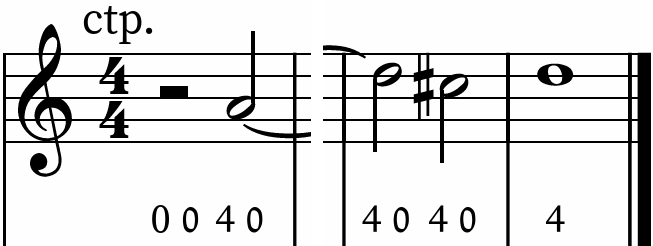
\includegraphics[height=0.9in]{Images/species_first_penult.png}
        \caption{First and penultimate measures in the $S$ array, \species{5}.}
        \label{fig:syncinfirstpenult}
    \end{figure}

    It is worth noting that the only silence occurs at the beginning of the counterpoint and is defined by the sequence $0-0$. This is the only time this sequence occurs. Another point, with the addition of this constraint, the last note of the counterpoint is necessarily linked to the fourth species, which has no particular impact because this note has the same role in all species, i.e. to be in perfect consonance with the \cfdot
\end{enumerate}

\section{Logic Implication of the Species Constraints}
Now that the solver knows when a note must be constrained by the rules of a species, it is necessary to represent this concept in the form of constraints.

\subsection{Generalization of the Species Implications}
For this, it is necessary that the previously established rules have the possibility of being activated only if the variables concerned by a rule are variables linked to the species to which the present rule belongs. In other words, a constraint of $x^{th}$ species on a set of variables $V$ must be true only and only if the variables $V$ are bound to notes belonging to this $x^{th}$ species. Unfortunately, this concept cannot be generalized to all the rules because some still apply when only part of the notes concerned is linked to the corresponding species. But an attempt at generalizing this idea can be written as such:

\begin{equation}
    \begin{gathered}
        \forall x \in \{3, 4\}, \forall cst_{x} \in Constraints(x), \forall V \in Variables(cst_{x})\\
        \left(\bigwedge_{\forall v \in V} IsS_{x}[v_{pos}]\right) \implies cst_{x}(V)\\
        \text{where }Constraints(x) \text{ is the set of constraints of the species }x,\\
        \text{and }Variables(cst_{x}) \text{ is the set of set of variables concerned by the constraint }cst_{x},\\
        \text{and }v_{pos} \text{ is the position of the } v \text{ related note in the array }Cp.\\
    \end{gathered}
\end{equation}

It will be seen in equation \ref{eq:syncopationvariation} in the next section that all the variables concerned by a constraint do not necessarily have to belong to the species in question. From the point of view of programming, each rule had to be re-examined according to its basic operation. This part of the work revealed some architectural concerns that the software was not well enough adapted to handle this new logic, but this will be discussed in section \ref{ch:future}.

Let's continue, in the current state of the program, florid counterpoint is considered to use either the third species or the fourth species. This means that a note has only three possible states: 0, 3 or 4. For example, rule \ref{rule:allcons} states by extension that notes in \emph{thesis} for the third species must be consonant but rule \ref{rule:arsiscons} states that they are the notes in \emph{arsis} for the fourth species which must be consonant. The two rules, hitherto distinct in two different species, result now in the fifth species in parallel.

Following the generalization:

\begin{equation} \label{eq:allcons5th}
    \begin{gathered}
        \forall V \in Variables(1.H1_{3})\quad
        \left(\bigwedge_{\forall v \in V} IsS_{3}[v_{pos}]\right) \implies 1.H1_{3}(V)\\
        \forall V \in Variables(4.H1_{4})\quad
        \left(\bigwedge_{\forall v \in V} IsS_{4}[v_{pos}]\right) \implies 4.H1_{4}(V)
    \end{gathered}
\end{equation}

And concretely:

\begin{equation} \label{eq:allcons5th}
    \begin{gathered}
        \forall j \in [0, m)\quad
        IsS_{3}[0, j] \implies (H[0, j] \in Cons)\\
        \forall j \in [0, m-1)\quad
        IsS_{4}[2, j] \implies (H[2, j] \in Cons)
    \end{gathered}
\end{equation}

It may seem simple but applying this logic to all the constraints of species 3 and 4 is not an easy task with the use of GiL which does not simply allow the addition of an implication on top of a constraint already written. The example above is one of the only cases where this is possible in this way but it must be understood that with GiL, which is only a precarious interface of Gecode, any intermediate step requires a new basic equation with only one operator. Mathematically, the equations would all follow the same notation which would basically just be a copy paste from the previous chapters. The rest of this chapter will therefore focus on the sometimes very specific relationships between species for certain rules that lead to slightly more complex constraints.

\subsection{Avoiding Multiple Same Final Solutions}
One might ask the question: what about notes where $S = 0$? These notes will not show up in the end user interface but the solver still calculates values for these notes. Does this mean that for a single solution on the user side there are a multitude of solutions on the solver side?

No, this is not the case because there is a constraint on the non-displayed notes, aka the non-constrained notes: they must be of the same value as the note of the next beat. In fact, it's the same as putting a fixed note on all the notes that don't appear, but for a branching issue, it's a little more efficient to work like that. The formulation is written as such:

\begin{equation}
    \begin{gathered}
        \forpm\quad
        IsS_{0}[\rho] \implies (Cp[\rho] = Cp[\rho + 1])
    \end{gathered}
\end{equation}

\section{Formalization of Inter-species Rules into Constraints}
Fux, before beginning the lesson of the fifth species, describes variations in syncopations and the introduction of eighth notes, without going into too much detail. \textcite[p.85]{GaPFr}

\begin{figure}[h]
    \centering
    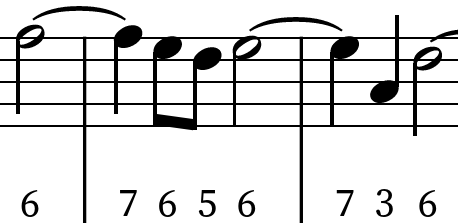
\includegraphics[height=0.8in]{Images/syncope_variations.png}
    \caption{Variation of a syncopation with quarter and eighth notes, \species{5}.}
    \label{fig:syncopevariation}
\end{figure}

This kind of variation is used a lot to get more interesting rhythms and melodies. This can be considered as an inter-species rule and requires more attention than the simple example given above (equation \ref{eq:allcons5th}). Figure \ref{fig:syncopevariation} shows two things:

\begin{enumerate}[wide]
    \item \label{rule:syncopationvariation} In relation to rule \ref{rule:dissolved}\footnote{A dissonant harmony in thesis must resolve in arsis with the next lower consonant harmony.}, the addition of quarter notes between the thesis and the arsis does not change the requirement to have an arsis consonance.
    \item \label{rule:crocheaddition} If the second eighth note is omitted, the melody does not move, which then implies that eighth notes can be used as mordents when the melodic interval between two beats is zero.
\end{enumerate}

How to formalize these concepts with the new species array system? For the observation \ref{rule:syncopationvariation}, it must be understood what is the role of the first quarter note in thesis. Since this is a quarter, shouldn't it be constrained by the third species? No, because this quarter note is part of the syncopation and is actually a $1/3$ of the latter\footnote{If a whole note is 1 unit long, then a half note lasts 1/2 unit and a quarter note lasts 1/4 unit. That type of syncopation then lasts 3/4 unit which is equivalent to three quarter notes.} played in arsis in the previous measure. This quarter note has no difference with the half note found in the original version of the syncope apart from its duration. So this note must be constrained by the fourth species. In fact, whether the duration of the note in thesis is one beat (quarter note) or two beats (half note) is only determined by whether or not a quarter note takes place in the second beat of the measure. To summarize the constraint that must be imposed: \textit{an arsis note, regardless of its species, must be the consonance just below the thesis note if the latter belongs to the fourth species}. This can be mathematically described by:

\begin{equation} \label{eq:syncopationvariation}
    \begin{gathered}
        \forall j \in [1, m-1)\\
        \lnot IsCons[0, j] \land IsS_{4}[0, j] \implies M^{2}_{brut}[0, j] \in \{-1, -2\} \land IsCons[2, j]
    \end{gathered}
\end{equation}\\

There is indeed a constraint which is applied to the notes in $[2, j]$ whereas the latter do not necessarily belong to the fourth species according to the $S$ array.\\

For the observation \ref{rule:crocheaddition}, Fux adds that:
\begin{quotation}
    "Furthermore, two eighths may occasionally be used in the next species; that is, on the second and fourth beats of the measure but never on the first and third." \textcite[p.63]{GaPEng}
\end{quotation}

\begin{figure}[h]
    \centering
    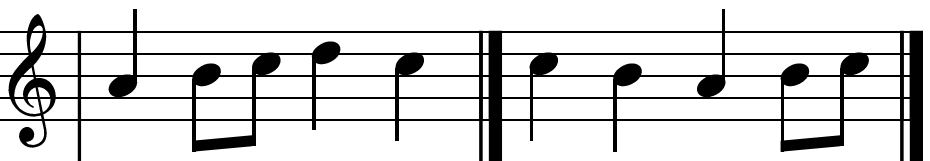
\includegraphics[width=3in]{Images/quarter_variations.png}
    \caption{Addition of eighth notes in second and fourth beat, \species{5}.}
    \label{fig:crocheaddition}
\end{figure}

One might be disappointed to learn that these rules are not added as constraints in the CSP but several points led to this.

First, even though the solver does not know anything about the second eighth note (the first one being considered as the original quarter), the algorithm that generates the rhythm (see next section) after the solver has run still creates eighth notes. The end user therefore obtains counterpoints with eighth notes.

Second, the second eighth note of the eighths-pair is not bound by any rule. This means that no new solution with eighth notes can be found by the solver except the original solution with a quarter note instead. The eighth note only completes an already existing leap of third or adds a mordent.

Third, the architecture of the program was not designed to handle a whole new note subdivision, especially compared to the almost non-existent interest.

However, the only constraint which changes, or rather which withdraws with this system of eighths is that the melodic interval is not obliged to be zero between the second and third beat and between the fourth and first beat of the next measure. Therefore, rule \ref{rule:notsamecons} which stated that two consecutive notes cannot be the same no longer applies at these positions.

\section{Parsing of the Species Array in Rhythm}
Rhythm species parsing occurs after the solver finds a solution. The parser therefore does not deal with Gecode variables but with values. Figure \ref{fig:rhythmdiagram} is a simplified diagram of the parser. It represents a recursive function that takes as input the entire ordered lists $Cp$ and $S$. This function outputs the final solution which will be shown to the user. The parser checks what is the next sequence of species and notes to find the corresponding note and associated duration. On the diagram, the notes are kept in the list \texttt{N} and the durations of the notes are kept in the list \texttt{R}. Once a sequence is found, it is removed from the lists $Cp$ and $S$ to be able to repeat the function again, this until the $Cp$ and $S$ lists are empty. This looks like a classic recursion pattern where the operation is performed on the head of the list and only the tail is kept for the next step. Here it is not necessarily a single element that is processed at a time but one to four elements. 
\newpage
The duration of notes in OpenMusic is represented as a fraction such that one unit represents an entire measure. Therefore, $1$ represents the duration of one whole note; $1/2$ that of a half note; $1/4$ that of a quarter note; etc. If the value is negative, then a silence is played instead of a note. Also, in the diagram, the notation \texttt{L=[x:]} means that the list \texttt{L} is stripped of its first \texttt{x} elements. This means that the previously checked sequence occupied the space of \texttt{x} beats in total. Finally, for the parser to work correctly, the last value of $S$ is replaced by $1$ to signify that it is a whole note.

% Example
% Cp = (72 72 72 72 72 71 71 69 67 69 69 69 69 68 68 69 69)
% S = (0 0 4 0 4 3 3 3 3 3 4 0 4 0 4 0 4)
% N = (72 71 69 71 69 67 69 71 69 68 69)
% R = (-1/2 3/4 1/8 1/8 1/4 1/4 1/4 1/8 1/8 1 1/2 1)
For example, if the values of the lists $Cp$ and $S$ are the following:
\begin{table}[!h]
    \centering
    \resizebox{\columnwidth}{!}{%
    \begin{tabular}{|c||cccc|cccc|cccc|cccc|c|}
    \hline
    $Cp$ & \textit{72} & \textit{72} & {\color[HTML]{3531FF} \textbf{72}} & \textit{72} & {\color[HTML]{3531FF} \textbf{72}} & {\color[HTML]{9A0000} \textbf{71}} & {\color[HTML]{9A0000} \textbf{71}} & {\color[HTML]{9A0000} \textbf{69}} & {\color[HTML]{9A0000} \textbf{67}} & {\color[HTML]{9A0000} \textbf{69}} & {\color[HTML]{3531FF} \textbf{69}} & \textit{69} & {\color[HTML]{3531FF} \textbf{69}} & \textit{68} & {\color[HTML]{3531FF} \textbf{68}} & \textit{69} & \textbf{69} \\
    \hline
    $S$  & \textit{0}  & \textit{0}  & {\color[HTML]{3531FF} \textbf{4}}  & \textit{0}  & {\color[HTML]{3531FF} \textbf{4}}  & {\color[HTML]{9A0000} \textbf{3}}  & {\color[HTML]{9A0000} \textbf{3}}  & {\color[HTML]{9A0000} \textbf{3}}  & {\color[HTML]{9A0000} \textbf{3}}  & {\color[HTML]{9A0000} \textbf{3}}  & {\color[HTML]{3531FF} \textbf{4}}  & \textit{0}  & {\color[HTML]{3531FF} \textbf{4}}  & \textit{0}  & {\color[HTML]{3531FF} \textbf{4}}  & \textit{0}  & \textbf{1} \\
    \hline
    \end{tabular}
    }
    \caption{Example of $Cp$ and $S$, \species{5}. Only the values in \textbf{bold} will be kept in the final solution.}
    \label{tab:exampleCpS}
\end{table}


Then the parsed output will be the following:
\begin{table}[!h]
    \centering
    % \resizebox{\columnwidth}{!}{%
    \begin{tabular}{|c||cc|cccc|cccc|c|c|}
    \hline
    \texttt{N} &      & {\color[HTML]{3531FF} \textbf{72}}  & {\color[HTML]{9A0000} \textbf{71}}  & 69  & {\color[HTML]{9A0000} \textbf{71}}  & {\color[HTML]{9A0000} \textbf{69}}  & {\color[HTML]{9A0000} \textbf{67}}  & {\color[HTML]{9A0000} \textbf{69}}  & 71  & {\color[HTML]{3531FF} \textbf{69}} & {\color[HTML]{3531FF} \textbf{68}}  & \textbf{69} \\
    \hline
    \texttt{R} & -1/2 & {\color[HTML]{3531FF} \textbf{3/4}} & {\color[HTML]{9A0000} \textbf{1/8}} & 1/8 & {\color[HTML]{9A0000} \textbf{1/4}} & {\color[HTML]{9A0000} \textbf{1/4}} & {\color[HTML]{9A0000} \textbf{1/4}} & {\color[HTML]{9A0000} \textbf{1/8}} & 1/8 & {\color[HTML]{3531FF} \textbf{1}}  & {\color[HTML]{3531FF} \textbf{1/2}} & \textbf{1}  \\
    \hline
    \end{tabular}
    % }
    \caption{Parsed output of table \ref{tab:exampleCpS}, \species{5}.}
    \label{tab:exampleNR}
\end{table}

Note that the sum of the absolute values of \texttt{R} will always be equal to $m$, the number of measures. On the user side, this would appear:

\begin{figure}[!h]
    \centering
    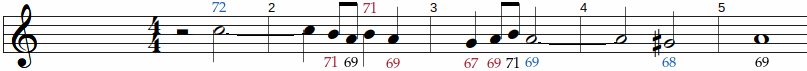
\includegraphics[width=5.2in]{Images/parser_example.png}
    \caption{Final outcome from table \ref{tab:exampleNR}, \species{5}.}
    \label{fig:parseruser}
\end{figure}

\begin{figure}[]
    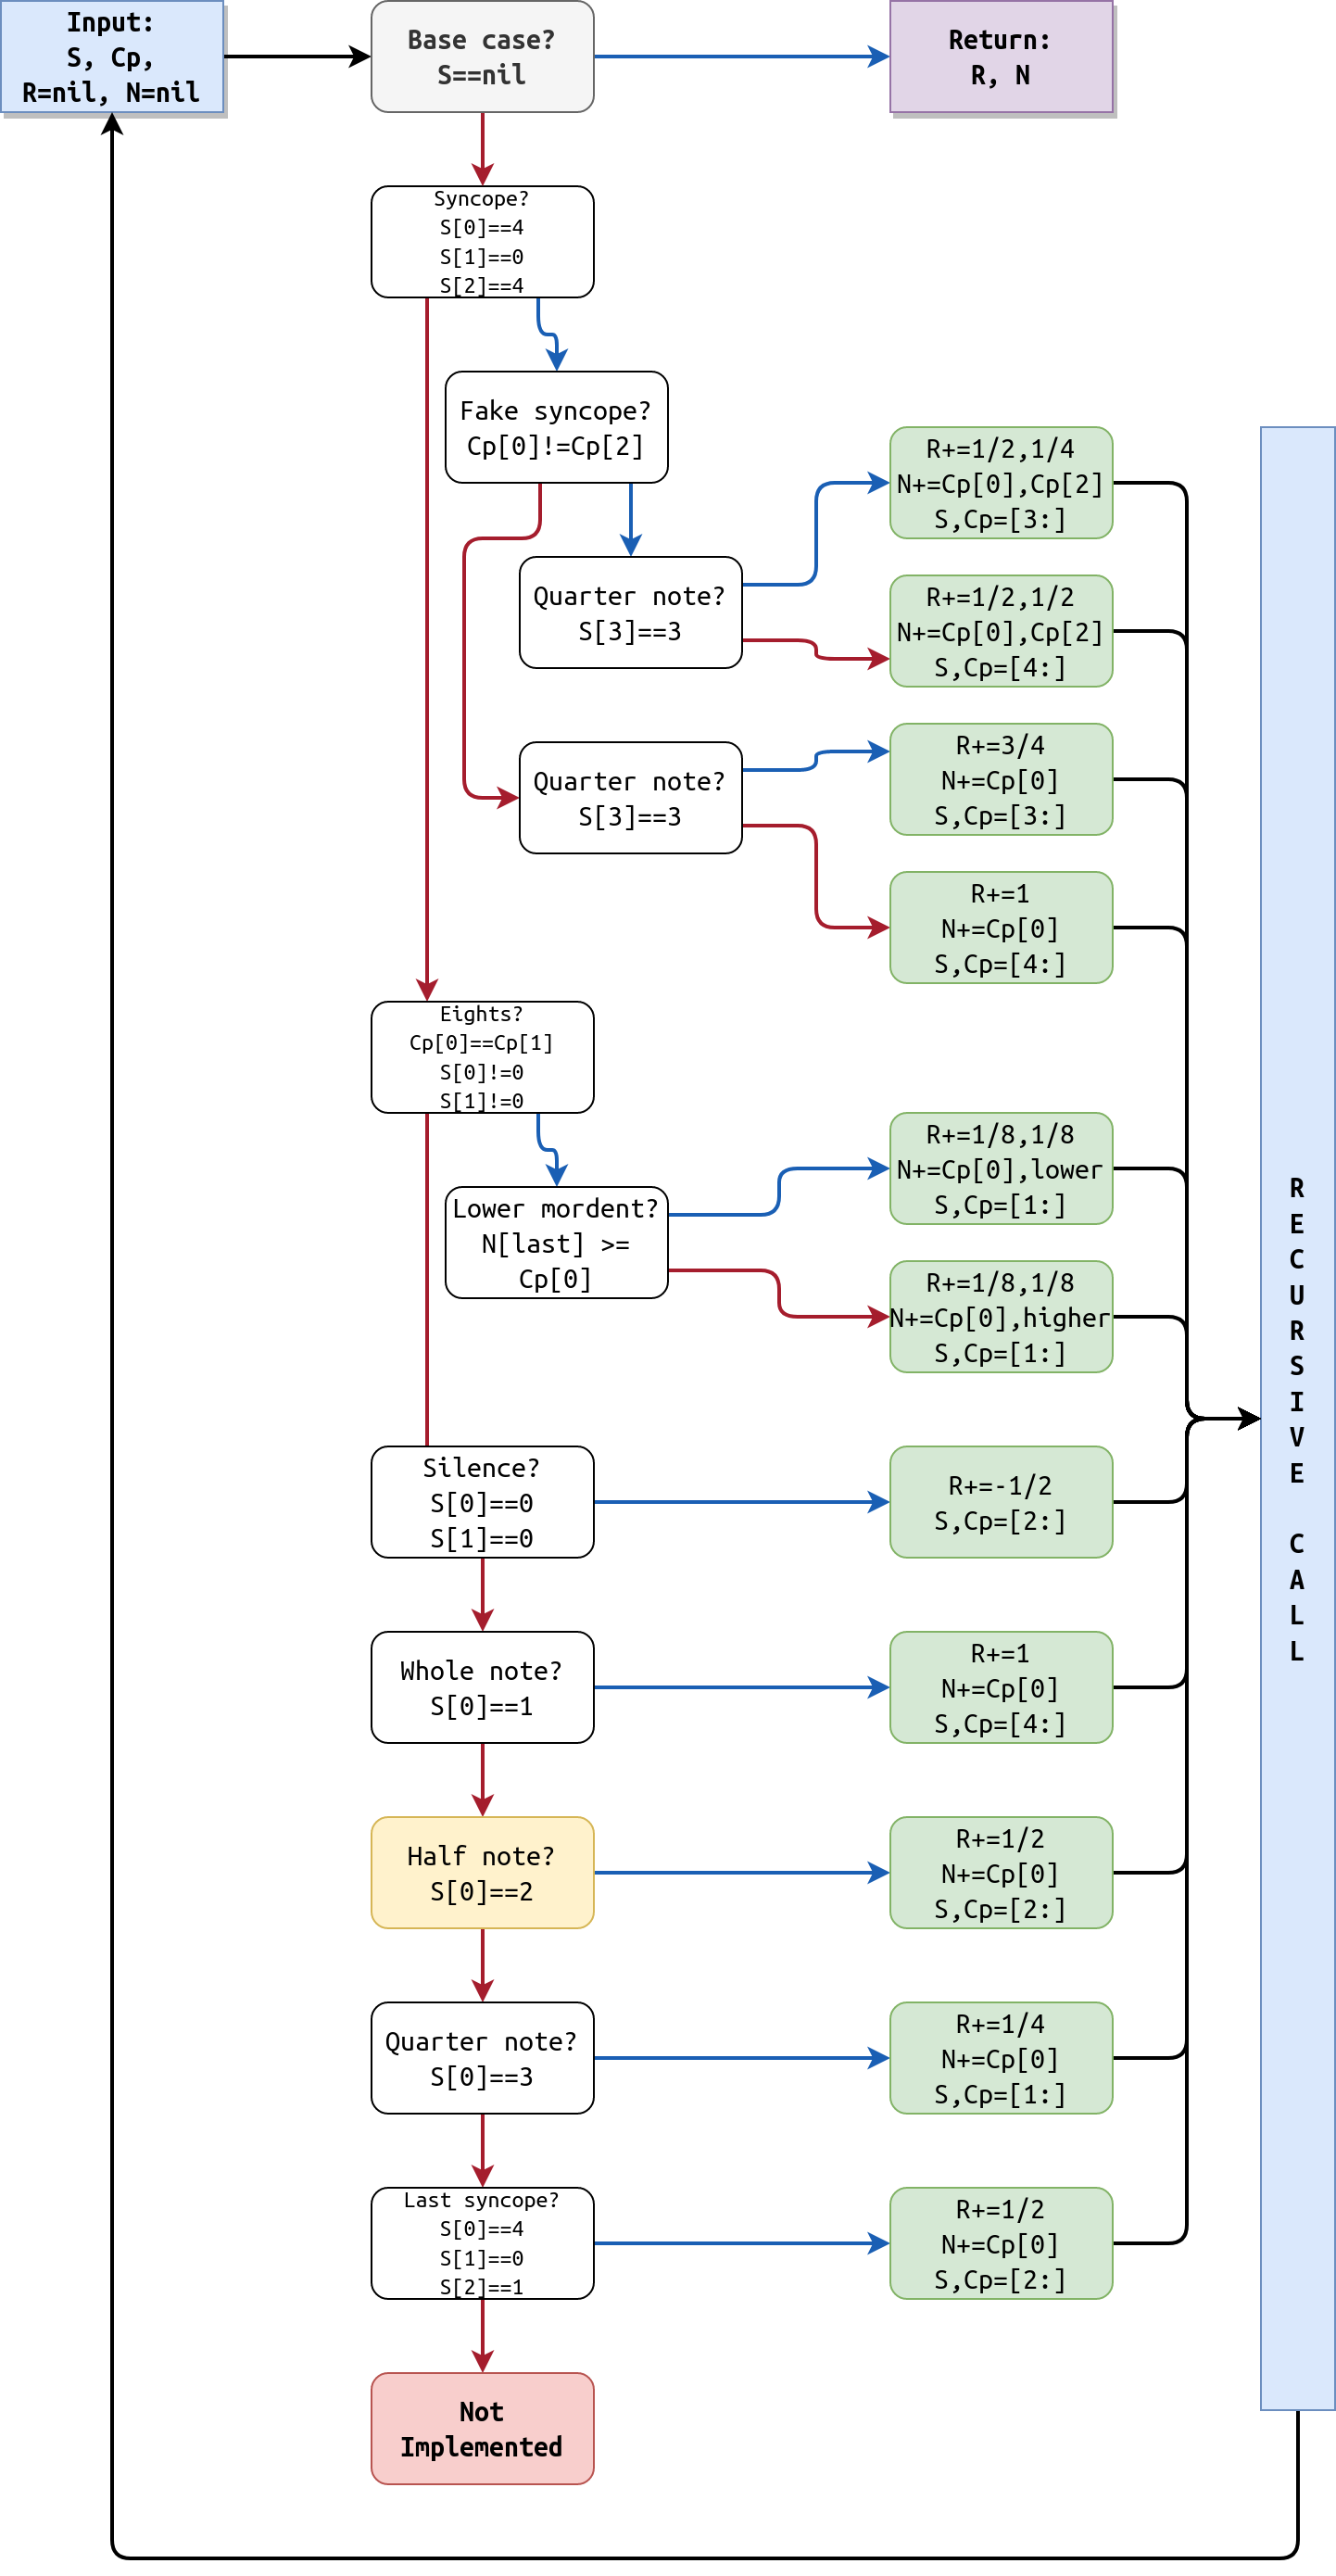
\includegraphics[scale=0.24, center]{Images/build_rhythmic_pattern.png}
    \caption{Rhythm species parser algorithm diagram, \species{5}. A \textcolor{red}{red arrow} means the test failed while a \textcolor{blue}{blue one} means it passed.}
    \label{fig:rhythmdiagram}
\end{figure}